\documentclass[fleqn]{article}

\usepackage{polski}
\usepackage[utf8]{inputenc}
\usepackage[polish]{babel}
\usepackage{parskip}
\usepackage{icomma}
\usepackage[a4paper,includeheadfoot,margin=1.27cm]{geometry}
\usepackage{float}
\usepackage{graphicx}
\usepackage{amsmath}
\usepackage[hypcap=true]{subcaption}
\usepackage{xcolor}
\usepackage{transparent}
\usepackage{listings}
\usepackage[colorlinks=true, linkcolor=blue, pdfborder={0 0 0}]{hyperref}

\renewcommand\thesection{\arabic{section}.}
\renewcommand\thesubsection{\alph{subsection})}
\renewcommand\thesubsubsection{}
\newcommand\square[1]{
	\fcolorbox{black}{#1}{\rule{0pt}{6pt}\rule{6pt}{0pt}}
}

\brokenpenalty=1000
\clubpenalty=1000
\widowpenalty=1000

\title{TM -- Laboratorium 3. \\ \large Licznik 8-bitowy – zerowanie, zliczanie w górę do zadanej wartości – kod NKB}
\author{Krystian Chachuła \\ Dawid Gruszczyński \\ Marcin Skrzypkowski}

\begin{document}

\maketitle

\setcounter{page}{0}
\thispagestyle{empty}

\pagebreak

\setcounter{page}{1}

\section{Wstęp}

Na trzecim laboratorium mieliśmy za zadanie, korzystając z modułu mikrokontrolera MSP430 oraz innych modułów SML-3, zaprojektować i zrealizować licznik zliczający w górę w kodzie NKB z możliwością asynchronicznego zerowania jego zawartości.
Sterowanie licznikiem miało odbywać się za pomocą dwóch przycisków (CLK aktywne zboczem oraz CLR aktywne poziomem).
Dodatkowym wymogiem zadania była realizacja programowej eliminacji drgań styków oraz obsługa przynajmniej jednego z przycisków z użyciem przerwań oraz ograniczanie maksymalnej wartości licznika z pomocą przełączników szesnastkowych.

Zaprojektowany przed laboratorium układ zbudowaliśmy z następujących układów SML-3:

\begin{itemize}
	\item \textbf{10\_PS1} (moduł zasilacza)
	\item \textbf{160\_7SEG2} (moduł wyświetlacza 7 segmentowego)
	\item \textbf{120\_IN8} (zestaw 8 monostabilnych wyłączników)
	\item \textbf{451\_IN\_4xHEX} (moduł przełączników szesnastkowych)
	\item \textbf{570\_MSP430F14x} (moduł mikrokontrolera Texas Instruments serii MSP430f14x lub F16x)
\end{itemize}

\section{Implementacja licznika}

Projektowanie rozpoczęliśmy od stworzenia grafu stanów, który przedstawiał ogólny schemat działania licznika.
%TODO ogarnąć grafuu

\begin{figure}[H]
	\centering
	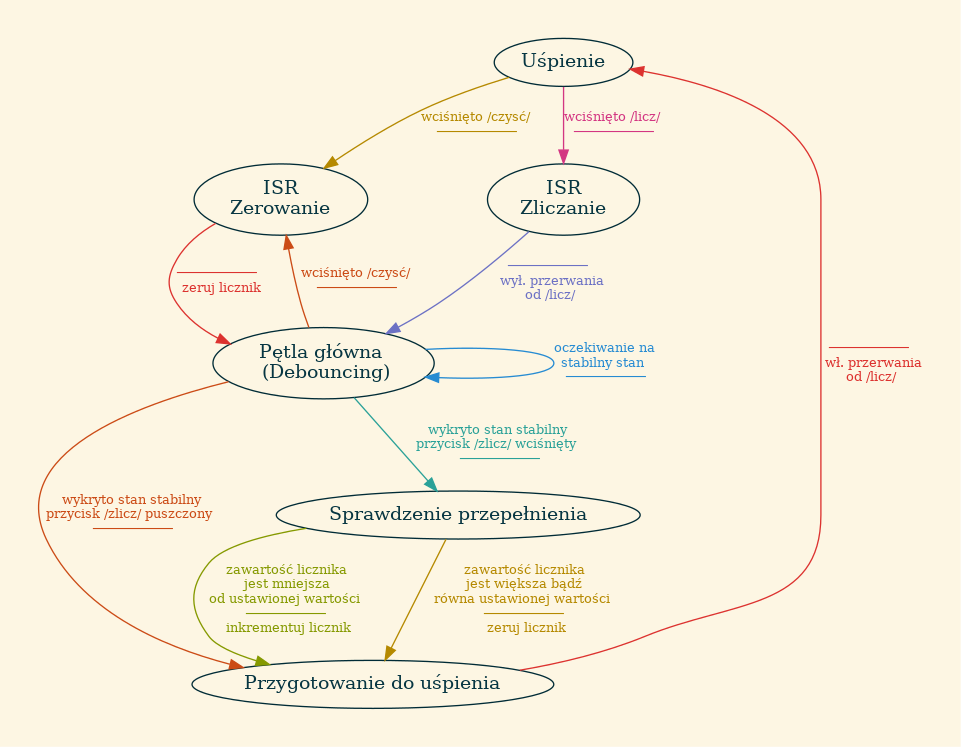
\includegraphics[width=\textwidth]{assets/graph.png}
	\caption{Graf automatu stanów}
	\label{fig:graph}
\end{figure}


Na początku pracy, mikrokontroler znajduje się w stanie uśpienia. Wybudzenie następuje tylko w przypadku wystąpienia przerwania z portu P1 (zbocze przycisku CLR) lub portu P2 (zbocze przycisku CLK). Następnie następuje przejście do obsługi zgłoszonego przerwania.

W przypadku przerwania od przycisku CLK, wyłączane są tylko przerwania generowane przez ten przycisk oraz trwale wybudzany jest mikrokontroler (przejście do pętli głównej programu). W przypadku przerwania od przycisku CLR zerowane jest wyjście licznika, zerowana jest zawartość rejestru służącego do usuwania drgań styków (rejestr R5) oraz wyłączane są przerwania od przycisku CLK (na czas trzymania wciśniętego przycisku CLR nie chcemy by istniała możliwość wywołania przerwania zliczającego). Wybudzany jest także trwale mikrokontroler.

Przerwania zliczające mogą być wywoływane tylko w momencie gdy mikrokontroler jest w stanie uśpienia, natomiast przerwania zerujące mogą być wywoływane w każdym miejscu poza sekcją krytyczną związaną z inkrementacją licznika. Przerwania nie mogą być zagnieżdżane. W pętli głównej programu, sprawdzane jest czy wciśnięty jest przycisk zerujący (w przypadku zerowania licznika blokujemy możliwość inkrementacji do momentu puszczeniu przycisku CLR) oraz czy wciśnięty jest przycisk zliczania (eliminacja drgań w przypadku inkrementacji licznika).

Eliminacja drgań odbywa się poprzez zliczanie do pewnej wartości za pomocą rejestru R5. Po pomyślnym przeczekaniu drgań następuje inkrementacja licznika. Proces eliminacji drgań może zostać przerwany przez wciśnięcie przycisku CLR, w takim przypadku licznik jest zerowany a proces inkrementacji zostaje przerwany. Po zakończeniu zerowania lub inkrementacji licznika, zerowany jest rejestr R5 oraz włączane są przerwania przycisku zliczającego, następnie mikrokontroler ponownie jest usypiany.

Na podstawie grafu powstał kod napisany w języku Assembly.



\section{Kod programu oraz jego opis}

\subsection{Blok Init}
		Na samym początku programu ustawiany jest wskaźnik stosu i wyłączany niepotrzebny w naszym obecnym projekcie watchdog, który nieobsłużony powodowałby niepożądany reset mikrokontrolera.
		W bloku \textit{Init} następuje ustawienie podstawowych flag przed rozpoczęciem działania licznika, a więc:
		\begin{itemize}
			\item następuje przypisanie przycisków zliczania i resetu do odpowiednich linii portów
			\item następuje odblokowanie przerwań pinów, do których są podłączone przyciski
			\item następuje wyzerowanie rejestru do debouncingu (\textit{R5}) oraz rejestru przechowującego pomocniczą flagę przerwania zerującego (\textit{R6})
			\item skonfigurowanie odpowiednich portów
		\end{itemize}

		W następnym bloku procesor od razu jest wprowadzany w stan oszczędzania energii LPM4 (wyłączone wszystkie zegary i procesor), z którego może być wybudzony tylko przerwaniem przycisku CLK bądź CLR. Po wybudzeniu następuje przejście do głównej części pętli.

\subsection{Procedura loop\_1}
		Pierwszą instrukcją, jaka jest wykonywana w tej procedurze, jest sprawdzenie wciśnięcia przycisku resetu. Jeśli jest on wciśnięty, następuje zapętlenie do loop\_1. Jeśli nie jest oznacza to, że albo został on puszczony, albo nie wystąpiło przerwanie zerujące a mikropocesor jest w trakcie sprawdzania dgrań przycisku zliczającego. W celu kontunuacji sprawdzana jest pomocnicza flaga znajdująca się w rejestrze R6, która ustawiana jest gdy wywoływane jest przerwanie zerujące. W sytuacji gdy jest ona równa 0, mikrokontroler może kontynuwać pracę, w przeciwnym przypadku następuje skok do procedury \textit{loop\_3} zakańczającej główną pętlę. Następnie, w celu eliminacji drgań styków, sprawdzany jest stan przycisku zliczającego. W przypadku gdy jest on puszczony przed doliczeniem do wartości testowej (ustaliliśmy wspólnie, że wystarczająca wartością będzie 0x04FF) następuje przeskok do \textit{loop\_3}. Jeśli debouncing zostanie zakończony pomyślnie, porównywana jest wartość aktualna licznika z wartością ustawioną na przełącznikach szesnastkowych. Jeżeli wartość na przełącznikach jest równa bądź mniejsza niż aktualna wartość licznika głównego, jest on resetowany i program skacze do procedury \textit{loop\_3}, w przeciwnym przypadku następuje inkremetacja licznika i przejście do procedury \textit{loop\_3}.

\subsection{Procedura loop\_3}
		W tej procedurze następuje czyszczenie rejestru debouncingu, reset flagi przerwania zliczającego i reset rejestru wystąpienia przerwania resetującego. Następnie odblokowane zostają przerwania od CLK i następuje powrót do stanu oszczędzania energii.

\subsection{Blok Przerwań}
		Po wystąpieniu przerwania od przycisku zliczania resetowane są bity odpowiedzialne za wprowadzanie mikrokontrolera w stan oszczędzania energii, aby procesor mógł przejść po jego obsłudze do pętli głównej. Blokowane są również przerwania od tego przycisku, aby podczas sprawdzania drgań nie były zgłaszane kolejne przerwania zliczające. Po powrocie z przerwania następuje przejście do procedury \textit{loop\_1}.

		Po wystąpieniu przerwania resetującego resetowany jest licznik główny, resetowane są flagi przerwań obu przycisków, aby po wyjściu z przerwania nie zgłaszały one przerwań, oraz wyłączane są przerwania zliczające, aby nie mogły być one wywoływane po wyjściu z obsługi przerwania resetującego (podczas gdy przycisk CLR jest wciśnięty nie chcemy by istaniła możliwość wywołania przerwania od przycisku CLK). Następnie resetujemy rejestr odpowiedzialny za eliminację drgań i ustawiana jest pomocnicza flaga oznajmiająca wystąpienie przerwania resetującego (zerowy bit rejestru \textit{R6}) i podobnie jak w przerwaniu przycisku zliczającego trwale wybudzamy mikrokontroler, by znowu móc pracować z pełną mocą. xD






\textbf{Kod programu:}



\lstinputlisting[lastline=55]{src/main.asm}

\lstinputlisting[firstline=56]{src/main.asm}

\pagebreak

\section{Podłączenie procesora}

Przyciski sterujące pracą licznika podłaczyliśmy do portów P1 oraz P2, (przycisk CLR do pinu 1 portu P1, ponieważ musi on posiadać większy priorytet, natomiast przycisk CLK do pinu 4 portu P2). Wyjściem licznika jest port P3 skonfigurowany jako wyjście, którego zawartość wyświetlana jest za pomocą modułu wyświetlacza 7 segmentowego. Do wczytywania wartości zadanej, do której ma zliczać licznik, wykorzystaliśmy port P4 skonfigurowany jako wejście. Jest on bezpośrednio podłaczony do modułu przełączników szesnatkowych.

\section{Możliwości rozwoju}

Możliwym udoskonaleniem zadania byłoby dodatkowe sprawdzanie poprawności odczytu wartości zadanej z modułu przełączników szesnastkowych. Odczyt w złym momencie może powodować przekłamania niektórych bitów spowodowane przełączaniem między pozycjami. Aby mieć pewność, że odczytany stan jest stabilny należy kilkukrotnie odczytać sygnał wejściowy na porcie P4 i sprawdzić czy odczytane wartości nie rożnią się między sobą. W przypadku różnic należy przeprowadzać ponowne odczyty aż do momentu uzyskania wartości stabilnej.

\end{document}
\grid
